\chapter{Specifikacija programske potpore}
		
	\section{Funkcionalni zahtjevi}
			
			\noindent \textbf{Dionici:}
			
			\begin{packed_enum}
				
				\item Tvrtke	
				\item Korisnici
				
				\begin{packed_enum}
					

					\item Vozač
					
				\end{packed_enum}
				
				\item Administrator
				\item Razvojni tim
			
			\end{packed_enum}
			
			\noindent \textbf{Aktori i njihovi funkcionalni zahtjevi:}
			

			\begin{packed_enum}
				\item  \underbar{Tvrtka (inicijator) može:}
				
				\begin{packed_enum}
					
					\item registrirati se u aplikaciji unoseći OIB, ime, adresu sjedišta, adresu e-pošte 
					\item prijaviti, pregledati, urediti i obrisati parkirališnu površinu

				\end{packed_enum}
				
				\item  \underbar{Neregistrirani korisnik (inicijator) može:}
				
				\begin{packed_enum}
					
					\item pregledati parkirališne površine
					\item stvoriti korisnički račun unoseći OIB, ime, prezime, adresu e-ppošte, broj registracije svojeg automobila i broj kreditne kartice
					\item dobiti ovlasti registriranog korisnika
					
				\end{packed_enum}
				
				\item  \underbar{Vozač (inicijator) može:}
				
				\begin{packed_enum}
			
					\item pregledati parkirališne površine
					\item pregledati i promijeniti osobne podatke
					\item pregledati, dodati, obrisati registarsku oznaku automobila u aplikaciju
					\item dobiti prijedlog najbližih parkirališnih površina za rezervaciju
					\item rezervirati parkirališno mjesto
					\item platiti rezervaciju
					\item pregledati, urediti, obrisati rezervacije

				\end{packed_enum}

				\item  \underbar{Administrator (inicijator) može:}
				
				\begin{packed_enum}

					\item vidjeti popis odabranih korisnika
					\item urediti i obrisati odabrane korisnike
					\item vidjeti popis odabranih tvrtki
					\item urediti i obrisati odabrane tvrtke
						
				\end{packed_enum}
				
				\item  \underbar{Baza podataka (inicijator) može:}
				
				\begin{packed_enum}
					
					\item pohranjuje sve podatke o korisnicima
					\item pohranjuje sve podatke o tvrtkama
				
				\end{packed_enum}
			\end{packed_enum}
\eject 
				
			\subsection{Obrasci uporabe}
				
					\noindent \underbar{\textbf{UC1  - Pregled parkirališnih površina}}
					\begin{packed_item}
						
						\item  \textbf{Glavni sudionik: } Vozač, neregistrirani korisnik
						\item  \textbf{Cilj:} Pregledati parkirališne površine
						\item  \textbf{Sudionici:} Baza podataka, Google maps
						\item  \textbf{Preduvjet:} -
						\item  \textbf{Opis osnovnog tijeka:}
						
						\item[] \begin{packed_enum}
							\item Karta je prikazana prilikom otvaranja aplikacije
							\item Korisnik na karti odabire parkirališnu površinu
							\item Prikazuju se informacije o odabranoj površini
						\end{packed_enum}
						
					\end{packed_item}
					\noindent \underbar{\textbf{UC2  - Registracija}}
					\begin{packed_item}
						
						\item  \textbf{Glavni sudionik: } Neregistrirani korisnik, Tvrtka
						\item  \textbf{Cilj:} Stvoriti korisnički račun
						\item  \textbf{Sudionici:} Baza podataka
						\item  \textbf{Preduvjet:} -
						\item  \textbf{Opis osnovnog tijeka:}
						
						\item[] \begin{packed_enum}
							\item Korisnik odabire opciju za registraciju (vozač ili tvrtka)
							\item Korisnik unosi potrebne korisničke podatke
						\end{packed_enum}
						
						\item  \textbf{Opis mogućih odstupanja:}
						
						\item[] \begin{packed_item}
							
							\item[2.a]  Odabir već zauzetog korisničkog imena i/ili e-pošte, unos korisničkog podataka u nedozvoljenom formatu ili pružanje neispravne e-pošte
							\item[] \begin{packed_enum}
								
								\item Sustav obavještava korisnika o neuspjelom upisu i vraća ga na stranicu za registraciju
								\item Korisnik mijenja potrebne podatke te završava unos ili odustaje od registracije
								
							\end{packed_enum}
						\end{packed_item}
					\end{packed_item}
					\noindent \underbar{\textbf{UC3  - Prijava u sustav}}
					\begin{packed_item}
						
						\item  \textbf{Glavni sudionik: } Vozač
						\item  \textbf{Cilj:} Dobiti pristup korisničkom sučelju
						\item  \textbf{Sudionici:} Baza podataka
						\item  \textbf{Preduvjet:} Registracija
						\item  \textbf{Opis osnovnog tijeka:}
						
						\item[] \begin{packed_enum}
							\item Unos korisničkog imena i lozinke
							\item Potvrda ispravnosti unesenih podataka
							\item Pristup korisničkim funkcijama
						\end{packed_enum}
						
						\item  \textbf{Opis mogućih odstupanja:}
						
						\item[] \begin{packed_item}
							
							\item[2.a]  Neispravno uneseni podatci
								\item[] \begin{packed_enum}
								
									\item Sustav obavještava korisnika o neuspjeloj prijavi
								
								\end{packed_enum}
						\end{packed_item}
					\end{packed_item}
					\noindent \underbar{\textbf{UC4  - Pregled osobnih podataka}}
					\begin{packed_item}
						
						\item  \textbf{Glavni sudionik: } Vozač, Tvrtka
						\item  \textbf{Cilj:} Pregledati osobne podatke
						\item  \textbf{Sudionici:} Baza podataka
						\item  \textbf{Preduvjet:} Korisnik je prijavljen
						\item  \textbf{Opis osnovnog tijeka:}
						
						\item[] \begin{packed_enum}
							\item Korisnik odabire opciju „osobni podatci“
							\item Aplikacija prikazuje osobne podatke korisnika
						\end{packed_enum}
						
					\end{packed_item}
					\noindent \underbar{\textbf{UC5  - Promjena osobnih podataka}}
					\begin{packed_item}
						
						\item  \textbf{Glavni sudionik: } Vozač, tvrtka
						\item  \textbf{Cilj:} Promijeniti osobne podatke
						\item  \textbf{Sudionici:} Baza podataka
						\item  \textbf{Preduvjet:} Korisnik je prijavljen
						\item  \textbf{Opis osnovnog tijeka:}
						
						\item[] \begin{packed_enum}
							\item Korisnik odabire opciju „osobni podatci“
							\item Korisnik mijenja svoje osobne podatke
							\item Korisnik sprema promjene
							\item Baza podataka se ažurira
						\end{packed_enum}
						
						\item  \textbf{Opis mogućih odstupanja:}
						
						\item[] \begin{packed_item}
							
							\item[2.a]  Korisnik promijeni svoje osobne podatke, ali je nešto neispravno uneseno
							\item[] \begin{packed_enum}
								
								\item Sustav obavještava korisnika da je nemoguće izmjeniti podatke prilikom odabira „Spremi promjene“
								
							\end{packed_enum}
						\end{packed_item}
					\end{packed_item}
					\noindent \underbar{\textbf{UC6  - Registracija auta}}
					\begin{packed_item}
						
						\item  \textbf{Glavni sudionik: } Vozač
						\item  \textbf{Cilj:} Registrirati automobil
						\item  \textbf{Sudionici:} Baza podataka
						\item  \textbf{Preduvjet:} Vozač je prijavljen
						\item  \textbf{Opis osnovnog tijeka:}
						
						\item[] \begin{packed_enum}
							\item Vozač odabire opciju „dodaj auto“
							\item Vozač unosi potrebne podatke
							\item Vozač prima obavijest o uspješnoj registraciji
						\end{packed_enum}
						
						\item  \textbf{Opis mogućih odstupanja:}
						
						\item[] \begin{packed_item}
							
							\item[2.a]  Unesena neispravna/već registrirana registracija
							\item[] \begin{packed_enum}
								
								\item Sustav obavijesti vozača da nije moguće registrirati auto, te ga vraća na stranicu za registraciju automobila
								\item Vozač mijenja podatke ili odustaje
								
							\end{packed_enum}
						\end{packed_item}
					\end{packed_item}
					\noindent \underbar{\textbf{UC7  - Pregled registriranih automobila}}
					\begin{packed_item}
						
						\item  \textbf{Glavni sudionik: } Vozač
						\item  \textbf{Cilj:} Pregledati registrirane automobile
						\item  \textbf{Sudionici:} Baza podataka
						\item  \textbf{Preduvjet:} Vozač je prijavljen
						\item  \textbf{Opis osnovnog tijeka:}
						
						\item[] \begin{packed_enum}
							\item Vozač odabire opciju „pregledaj aute“
							\item Aplikacija prikazuje automobile koje je vozač prijašnje unio ako postoje
						\end{packed_enum}
						
					\end{packed_item}
					\noindent \underbar{\textbf{UC8  - Brisanje registriranih automobila}}
					\begin{packed_item}
						
						\item  \textbf{Glavni sudionik: } Vozač
						\item  \textbf{Cilj:} Obrisati registrirane automobile
						\item  \textbf{Sudionici:} Baza podataka
						\item  \textbf{Preduvjet:} Vozač je prijavljen
						\item  \textbf{Opis osnovnog tijeka:}
						
						\item[] \begin{packed_enum}
							\item Vozač odabere opciju „pregledaj aute“
							\item Vozač odabire auto koje želi obrisati i stisne  „obriši“
							\item Baza podataka se ažurira
						\end{packed_enum}
					\end{packed_item}
					\noindent \underbar{\textbf{UC9 - Rezervacija parkirališnog mjesta}}
					\begin{packed_item}
						
						\item  \textbf{Glavni sudionik: } Vozač
						\item  \textbf{Cilj:} Rezervirati parking mjesto
						\item  \textbf{Sudionici:} Baza podataka,  Google maps
						\item  \textbf{Preduvjet:} Vozač je prijavljen
						\item  \textbf{Opis osnovnog tijeka:}
						
						\item[] \begin{packed_enum}
							\item Vozač odabere opciju „Napravi rezervaciju“
							\item Sustav pronalazi vozaču najbližu parkirališnu površinu
							\item Vozač odabire ponuđenu parkirališnu površinu ili sam na karti pronalazi drugu
							\item Vozač odabire vozilo za koje želi napraviti rezervaciju
							\item Vozač ispuni potrebne informacije za rezervaciju
							\item Vozač odabire opciju „Potvrdi rezervaciju“
							\item Sustav naplati rezervaciju
						\end{packed_enum}
						
						\item  \textbf{Opis mogućih odstupanja:}
						
						\item[] \begin{packed_item}
							
							\item[3.a]  Na parkingu nema slobodnog mjesta
							\item[] \begin{packed_enum}
								
								\item Sustav obavještava vozača da nema slobodnog mjesta i daje korisniku opciju mijenjanja datuma rezervacije
								
							\end{packed_enum}
						\end{packed_item}
					\end{packed_item}
				
					\noindent \underbar{\textbf{UC10  - Pregled aktivnih rezervacija}}
					\begin{packed_item}
						
						\item  \textbf{Glavni sudionik: } Vozač
						\item  \textbf{Cilj:} Pregledati aktivne rezervacije
						\item  \textbf{Sudionici:} Baza podataka
						\item  \textbf{Preduvjet:} Vozač je prijavljen
						\item  \textbf{Opis osnovnog tijeka:}
						
						\item[] \begin{packed_enum}
							\item Vozač odabire opciju „Pregledaj rezervacije“
							\item Sustav prikaže vozaču aktivne rezervacije ukoliko takve postoje
						\end{packed_enum}
					
					\end{packed_item}
					
							
					\noindent \underbar{\textbf{UC11  - Brisanje aktivnih rezervacija}}
					\begin{packed_item}
						
						\item  \textbf{Glavni sudionik: } Vozač
						\item  \textbf{Cilj:} Obrisati rezervaciju
						\item  \textbf{Sudionici:} Baza podataka
						\item  \textbf{Preduvjet:} Vozač je prijavljen i napravio je barem jednu rezervaciju
						\item  \textbf{Opis osnovnog tijeka:}
						
						\item[] \begin{packed_enum}
							\item Vozač odabire opciju „Pregledaj rezervacije“
							\item Sustav prikaže listu rezervacija vozača
							\item Vozač odabire opciju „Obriši rezervaciju“
							\item Rezervacija se briše iz baze podataka
							\item Vozaču se vraćaju novci ako ima neiskorištenih rezervacija
						\end{packed_enum}
						
						\item  \textbf{Opis mogućih odstupanja:}
						
						\item[] \begin{packed_item}
							
							\item[4.a]  Greška prilikom refundiranja novca
							\item[] \begin{packed_enum}
								
								\item Sustav obavještava vozača da je došlo do greške prilikom refundiranja novca na njegov račun, te se odustaje od brisanja rezervacije.
								
							\end{packed_enum}
						\end{packed_item}
						
					\end{packed_item}
					\noindent \underbar{\textbf{UC12 - Prijava parkirališne površine}}
					\begin{packed_item}
						
						\item  \textbf{Glavni sudionik: } Tvrtka
						\item  \textbf{Cilj:} Prijaviti parking objekt
						\item  \textbf{Sudionici:} Baza podataka
						\item  \textbf{Preduvjet:} Tvrtka je prijavljena
						\item  \textbf{Opis osnovnog tijeka:}
						
						\item[] \begin{packed_enum}
							\item Tvrtka odabire opciju „Dodaj parkirališnu površinu“
							\item Unos podataka o parkirališnoj površini
							\item Tvrtka unese sve podatke i odabire „Spremi“
							\item Ažurira se baza podataka
						\end{packed_enum}
						
						\item  \textbf{Opis mogućih odstupanja:}
						
						\item[] \begin{packed_item}
							
							\item[2.a]  Unesen neispravan/već prijavljen parking
							\item[] \begin{packed_enum}
								
								\item Sustav obavijesti korisnika da nije moguće prijaviti parking te ga vraća na stranicu za prijavu parkirališne površine
								\item Korisnik mijenja podatka ili odustaje
								
							\end{packed_enum}
						\end{packed_item}
					\end{packed_item}
					\noindent \underbar{\textbf{UC13  - Pregled prijavljenih parkirališnih površina}}
					\begin{packed_item}
						
						\item  \textbf{Glavni sudionik: } Tvrtka
						\item  \textbf{Cilj:} Pregled prijavljenih parkirališnih površina
						\item  \textbf{Sudionici:} Baza podataka
						\item  \textbf{Preduvjet:} Tvrtka je prijavljena i postoji prijavljena parkirališna površina
						\item  \textbf{Opis osnovnog tijeka:}
						
						\item[] \begin{packed_enum}
							\item Korisnik odabire opciju „Upravljaj parkirališnim površinama“
							\item Otvara se lista prijavljenih parkirališnih površina
						\end{packed_enum}
						
					\end{packed_item}
					
					\noindent \underbar{\textbf{UC14  - Brisanje parkirališnih površina}}
					\begin{packed_item}
						
						\item  \textbf{Glavni sudionik: } Tvrtka
						\item  \textbf{Cilj:} Obrisati parkirališnu površinu
						\item  \textbf{Sudionici:} Baza podataka
						\item  \textbf{Preduvjet:} - Tvrtka je prijavljena i ima barem jedan prijavljeni parkirališnu površinu
						\item  \textbf{Opis osnovnog tijeka:}
						
						\item[] \begin{packed_enum}
							\item Korisnik odabire opciju „Upravljaj parkirališnim površinama“
							\item Sustav prikaže listu prijavljenih parkirališnih površina
							\item Korisnik briše željenu parkirališnu površinu
							\item Ažurira se baza podataka

						\end{packed_enum}
						
					\end{packed_item}
					\noindent \underbar{\textbf{UC15  - Pregled vozača}}
					\begin{packed_item}
						
						\item  \textbf{Glavni sudionik: }Administrator
						\item  \textbf{Cilj:}  Vidjeti popis vozača
						\item  \textbf{Sudionici:} Baza podataka
						\item  \textbf{Preduvjet:} - Administrator prijavljen
						\item  \textbf{Opis osnovnog tijeka:}
						
						\item[] \begin{packed_enum}
							\item Administrator odabire opciju „Popis vozača“
							\item Pojavi se lista vozača
						\end{packed_enum}
						
					\end{packed_item}
					\noindent \underbar{\textbf{UC16  - Uređivanje vozača}}
					\begin{packed_item}
						
						\item  \textbf{Glavni sudionik: } Administrator
						\item  \textbf{Cilj:} Urediti vozače
						\item  \textbf{Sudionici:} Baza podataka
						\item  \textbf{Preduvjet:} Administrator prijavljen i postoji barem jedan korisnik
						\item  \textbf{Opis osnovnog tijeka:}
						
						\item[] \begin{packed_enum}
							\item Administrator pronalazi željenog vozača i odabire opciju „Uredi“
							\item Sustav prikazuje podatke o odabranom vozaču
							\item Administrator upravlja njegovim podacima
							\item Ažurira se baza podataka
						\end{packed_enum}
						
					\end{packed_item}
					\noindent \underbar{\textbf{UC17  - Brisanje vozača}}
					\begin{packed_item}
						
						\item  \textbf{Glavni sudionik: } Admin
						\item  \textbf{Cilj:}  sudionik: Obrisati odabranog vozača
						\item  \textbf{Sudionici:} Baza podataka
						\item  \textbf{Preduvjet:} Admin prijavljen i postoji barem jedan korisnik
						\item  \textbf{Opis osnovnog tijeka:}
						
						\item[] \begin{packed_enum}
							\item Administrator pronalazi željenog vozača i odabire opciju „Obriši“
							\item Vozač se obriše
							\item Ažurira se baza podataka
						\end{packed_enum}
						
					\end{packed_item}
					\noindent \underbar{\textbf{UC18  - Pregled tvrtki}}
					\begin{packed_item}
						
						\item  \textbf{Glavni sudionik: } Admin
						\item  \textbf{Cilj:} Vidjeti popis odabranih tvrtki
						\item  \textbf{Sudionici:} Baza podataka
						\item  \textbf{Preduvjet:} Admin prijavljen
						\item  \textbf{Opis osnovnog tijeka:}
						
						\item[] \begin{packed_enum}
							\item Administrator odabire opciju „Popis tvrtki“
							\item Pojavi se lista s odabranim tvrtkama
						\end{packed_enum}
						
					\end{packed_item}
					\noindent \underbar{\textbf{UC19  - Uređivanje odabranih tvrtki}}
					\begin{packed_item}
						
						\item  \textbf{Glavni sudionik: } Administrator
						\item  \textbf{Cilj:} Urediti odabrane tvrtke
						\item  \textbf{Sudionici:} Baza podataka
						\item  \textbf{Preduvjet:} Administrator prijavljen i postoji barem jedna tvrtka
						\item  \textbf{Opis osnovnog tijeka:}
						
						\item[] \begin{packed_enum}
							\item Administrator pronalazi željenu tvrtku i odabire opciju „Uredi“
							\item Sustav prikazuje podatke o odabranoj tvrtki
							\item Administrator upravlja njezinim podacima
							\item Ažurira se baza podataka
						\end{packed_enum}
						
					\end{packed_item}
					\noindent \underbar{\textbf{UC20  - Brisanje odabranih tvrtki}}
					\begin{packed_item}
						
						\item  \textbf{Glavni sudionik: } Administrator
						\item  \textbf{Cilj:} Obrisati odabrane tvrtke
						\item  \textbf{Sudionici:} Baza podataka
						\item  \textbf{Preduvjet:} - Administrator je prijavljen i postoji barem jedan korisnik
						\item  \textbf{Opis osnovnog tijeka:}
						
						\item[]	\begin{packed_enum}
							\item Administrator odabire željenu tvrtku i odabire opciju „Obriši“
							\item Tvrtka se obriše
							\item Ažurira se baza podataka
						\end{packed_enum}
					
					\end{packed_item}
							
			\eject		
			
				\subsubsection{Dijagrami obrazaca uporabe}
				
					%unos slike
					\begin{figure}[H]
						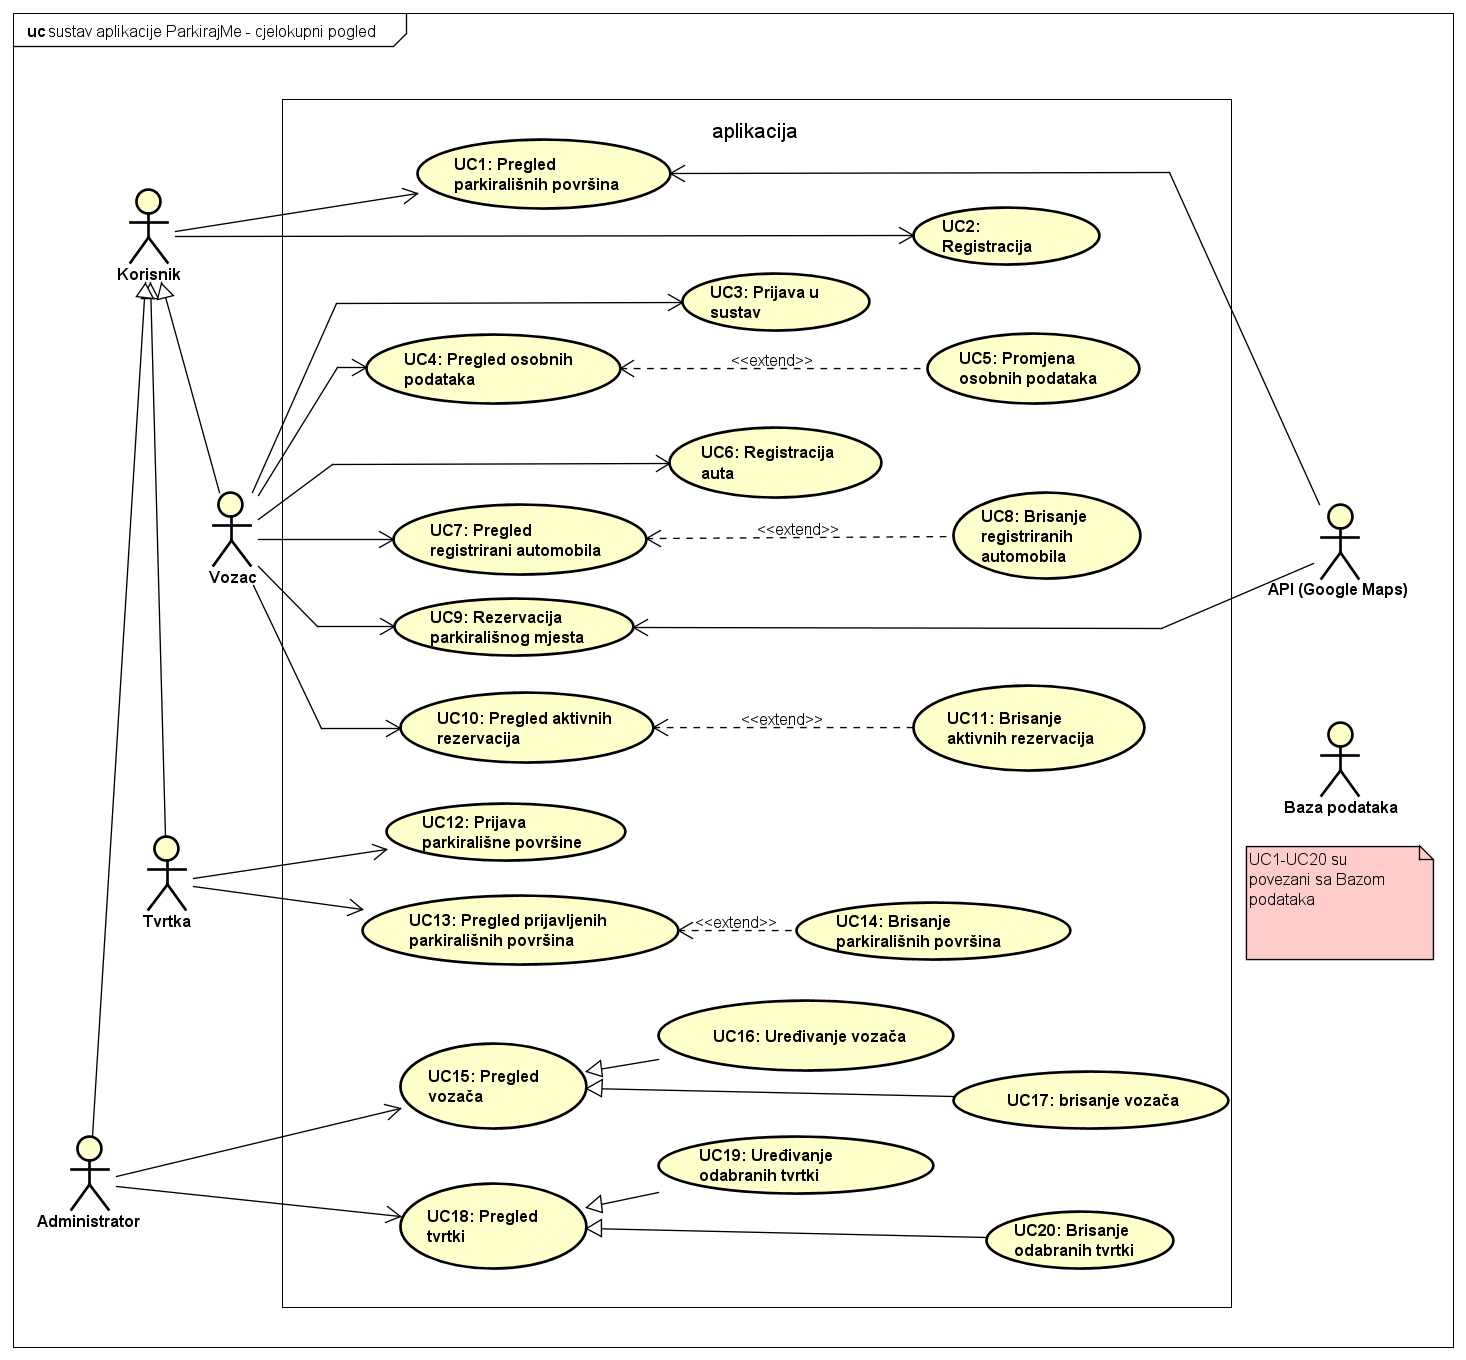
\includegraphics[scale=0.4]{dijagrami/cjelokupni_pogled.png} %veličina slike u odnosu na originalnu datoteku i pozicija slike
						\centering
						\caption{Cjelokupni pogled}
						\label{fig:promjene}
					\end{figure}
				
					%unos slike
					\begin{figure}[H]
						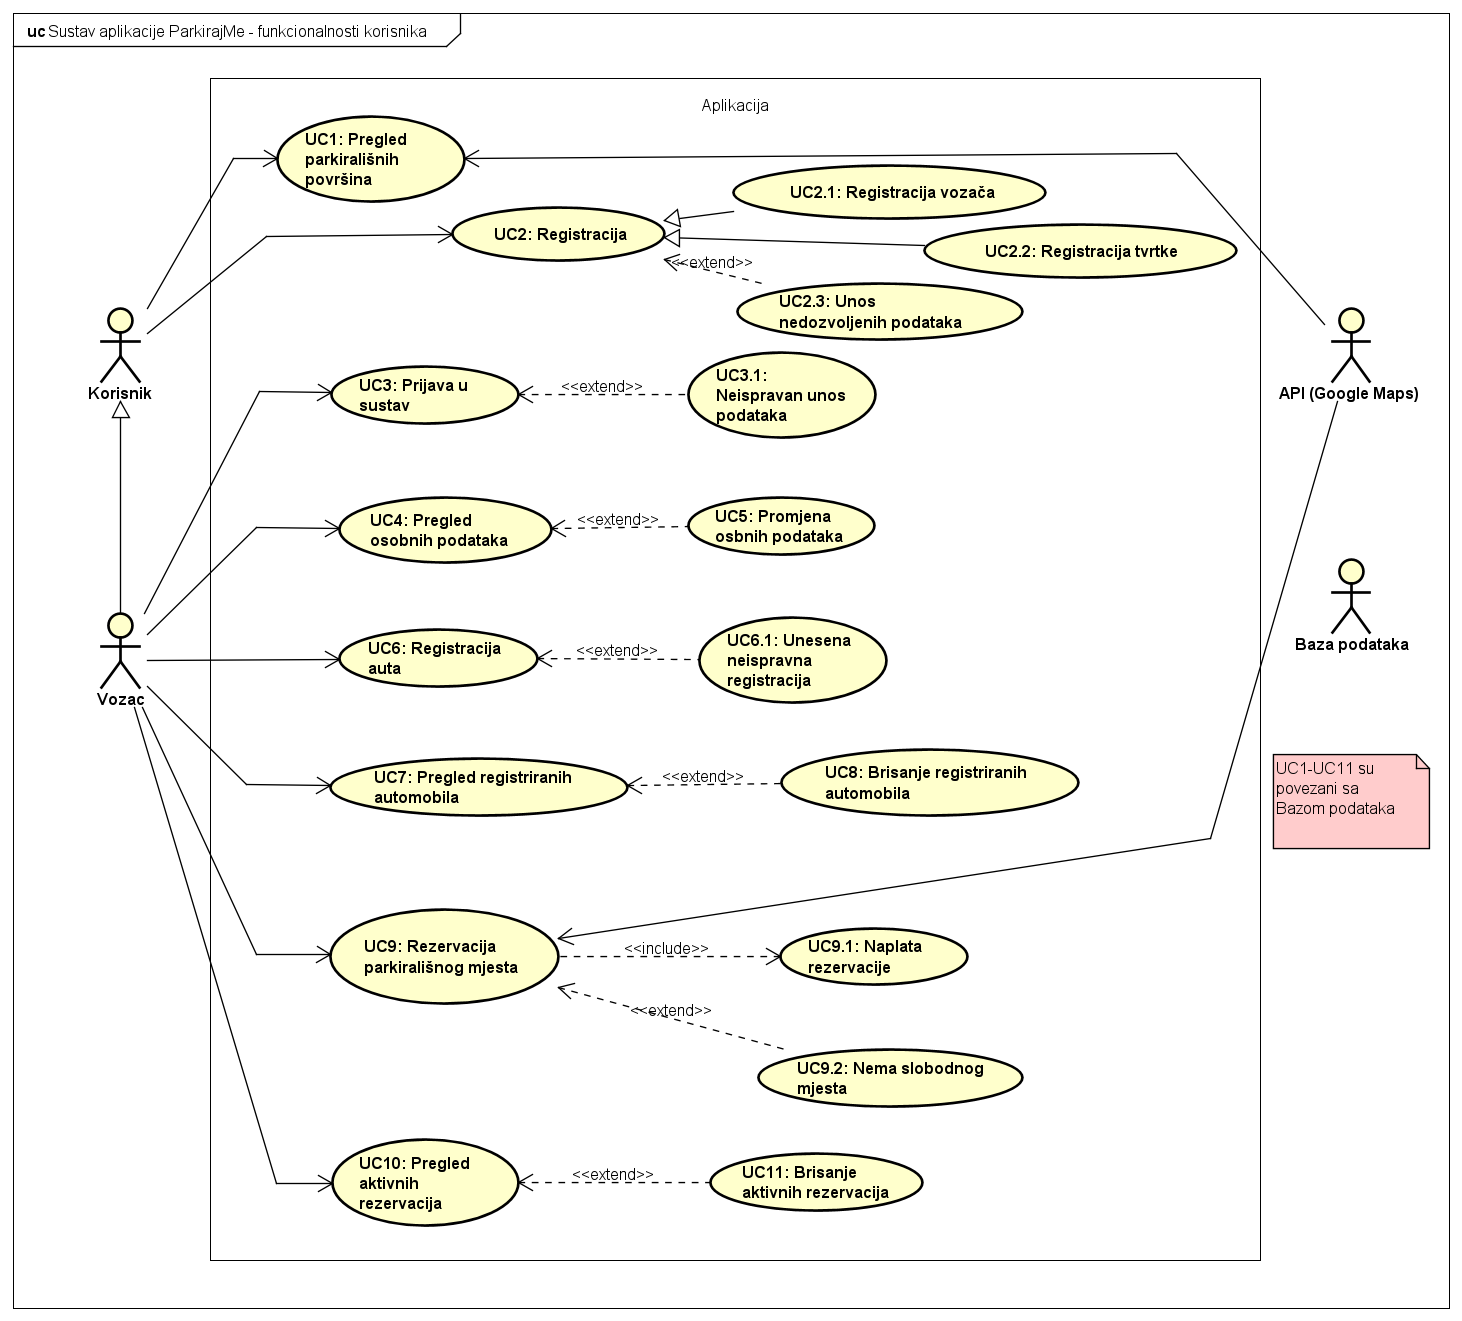
\includegraphics[scale=0.4]{dijagrami/funkcionalnosti_korisnika.png} %veličina slike u odnosu na originalnu datoteku i pozicija slike
						\centering
						\caption{Funkcionalnosti korisnika}
						\label{fig:promjene}
					\end{figure}
				
					%unos slike
					\begin{figure}[H]
						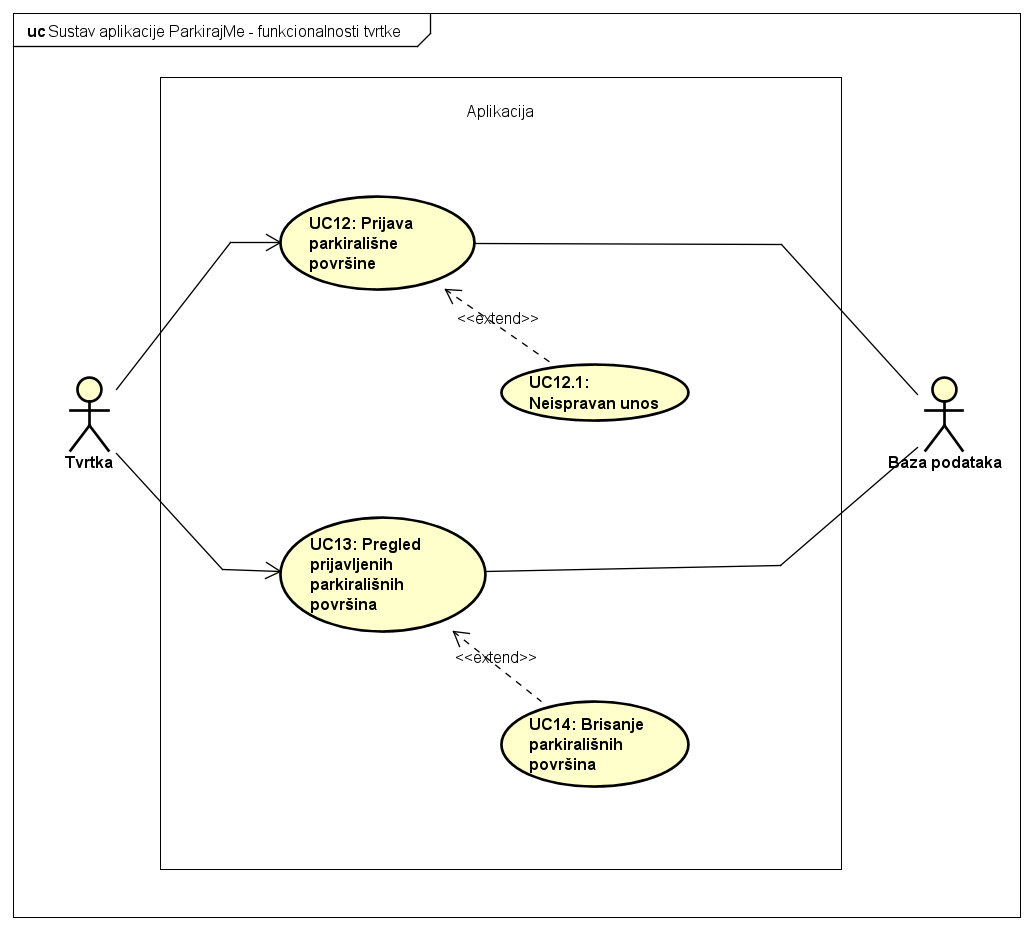
\includegraphics[scale=0.55]{dijagrami/funkcionalnosti_tvrtke.png} %veličina slike u odnosu na originalnu datoteku i pozicija slike
						\centering
						\caption{Funkcionalnosti tvrtke}
						\label{fig:promjene}
					\end{figure}
				
					%unos slike
					\begin{figure}[H]
						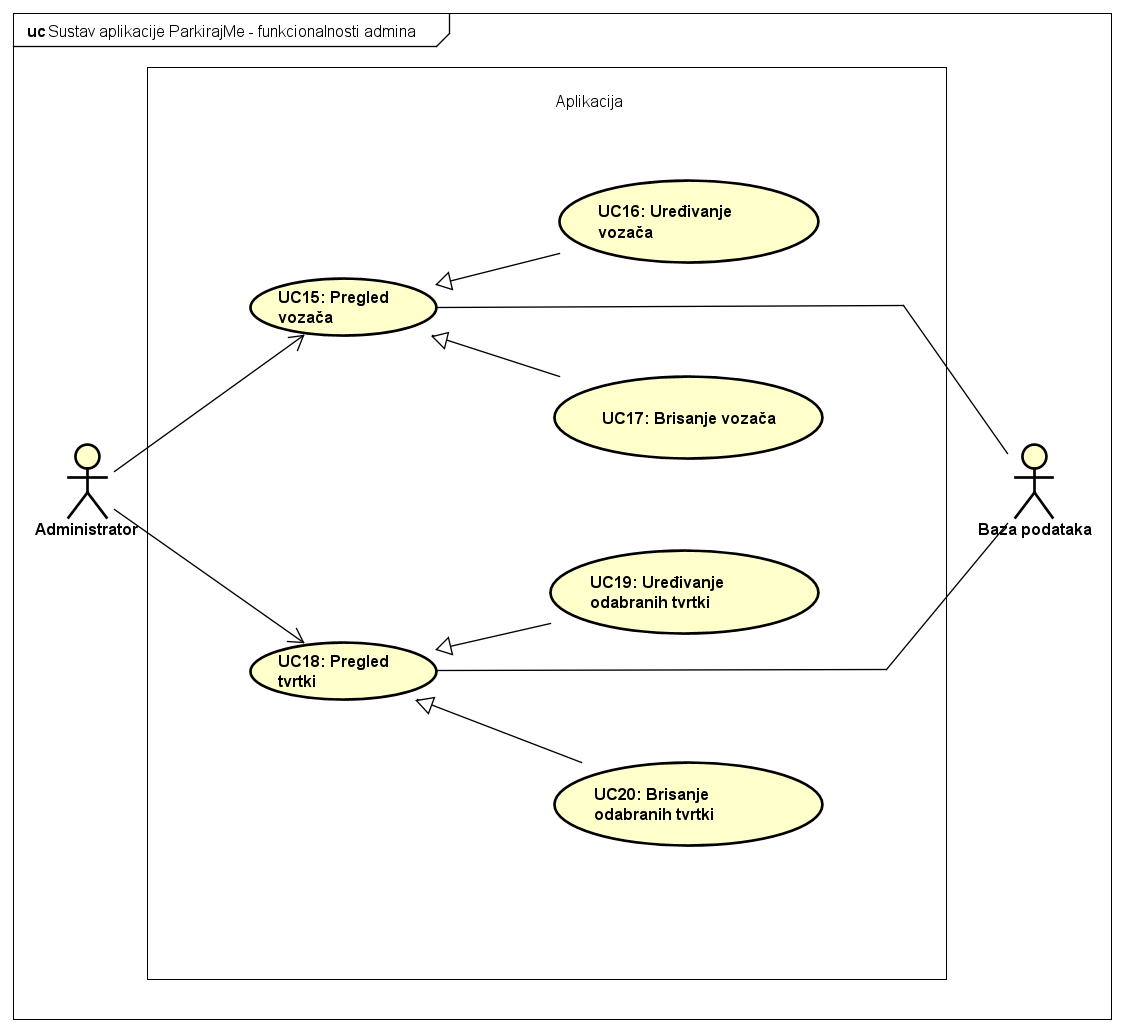
\includegraphics[scale=0.5]{dijagrami/funkcionalnosti_admina.png} %veličina slike u odnosu na originalnu datoteku i pozicija slike
						\centering
						\caption{Funkcionalnosti admina}
						\label{fig:promjene}
					\end{figure}				
				\eject		
				
			\subsection{Sekvencijski dijagrami}
				
				
				\noindent {\textbf{Obrazac uporabe UC2 - Registracija}}\\
				Korisnik bira jednu od dvije opcije registracije: "Registriraj se kao korisnik" ili "Registriraj se kao tvrtka". Nakon odabira željene registracije aplikacija ga traži unos potrebnih podataka. Aplikacija provjerava jesu li sva polja popunjena i je li format unesenih podataka ispravan (broj znamenki OIB-a,format adrese e-pošte...). Nakon toga aplikacija pristupa bazi podataka i provjerava jedinstvenost unesenih podataka. Ako su podaci ispravni, ovisno o vrsti registracije, stvara se novi vozač ili korisnički račun tvrtke te se podaci pohranjuju u bazu podataka. Ako su uneseni podaci neispravni, korisnik prima obavijest i aplikacija ga vraća na glavni izbornik.
	

				\begin{figure}[H]
					\includegraphics[scale=0.5]{dijagrami/Sekvencijski dijagram - Registracija.png} %veličina slike u odnosu na originalnu datoteku i pozicija slike
					\centering
					\caption{Sekvencijski dijagram - Registracija}
					\label{fig:promjene}
				\end{figure}	
			
				\newpage
				\noindent {\textbf{Obrazac uporabe UC11 - Brisanje aktivnih rezervacija}}\\
				Vozač odabire opciju "pregledaj rezervacije" nakon čega poslužitelj pristupa bazi podataka i dohvaća listu svih vozačevih rezervacija. Vozač odabire jednu rezervaciju koju želi obrisati i klikom na gumb "obriši" rezervacije se briše. Ako rezervacija još nije iskorištena, aplikacija uplaćuje cijenu rezervacije na vozačev račun i briše ju iz baze podatatka. Ako je rezervacija već iskorištena, aplikacija ju uklanja iz baze podataka. Nakon brisanja rezervacije, korisnik se vraća na glavni izbornik.
			\\
				
				\begin{figure}[H]
					\includegraphics[scale=0.5]{dijagrami/Sekvencijski dijagram -brisanje aktivnih rezervacija.png} %veličina slike u odnosu na originalnu datoteku i pozicija slike
					\centering
					\caption{Sekvencijski dijagram - Brisanje aktivnih rezervacija}
					\label{fig:promjene}
				\end{figure}	
			
				\newpage
			\noindent {\textbf{Obrazac uporabe UC12 - Prijava parkirališne površine}}\\
			Korisnik koji je prijavljen sa korisničkim računom tvrtke može prijaviti novu parkirališnu površinu. Odabirom opcije "Dodaj parkirališnu površinu" otvara se izbornik koji od korisnika traži unos podataka. Klikom miša na karti, korisnik postavlja marker na željenu lokaciju i time označava mjesto parkirališne površine. Google Karte prosljeđuju koordinate lokacije aplikaciji te aplikacija prikazuje koordinate korisniku. Ako korisnik nije zadovoljan odabranim koordinatama, klikom na opciju "restartaj marker" može ponovno označiti lokaciju na karti. Nakon što korisnik unese ostale tražene podatke i odabere "spremi lokaciju", podaci se spremaju u bazu podataka.
			
			\begin{figure}[H]
				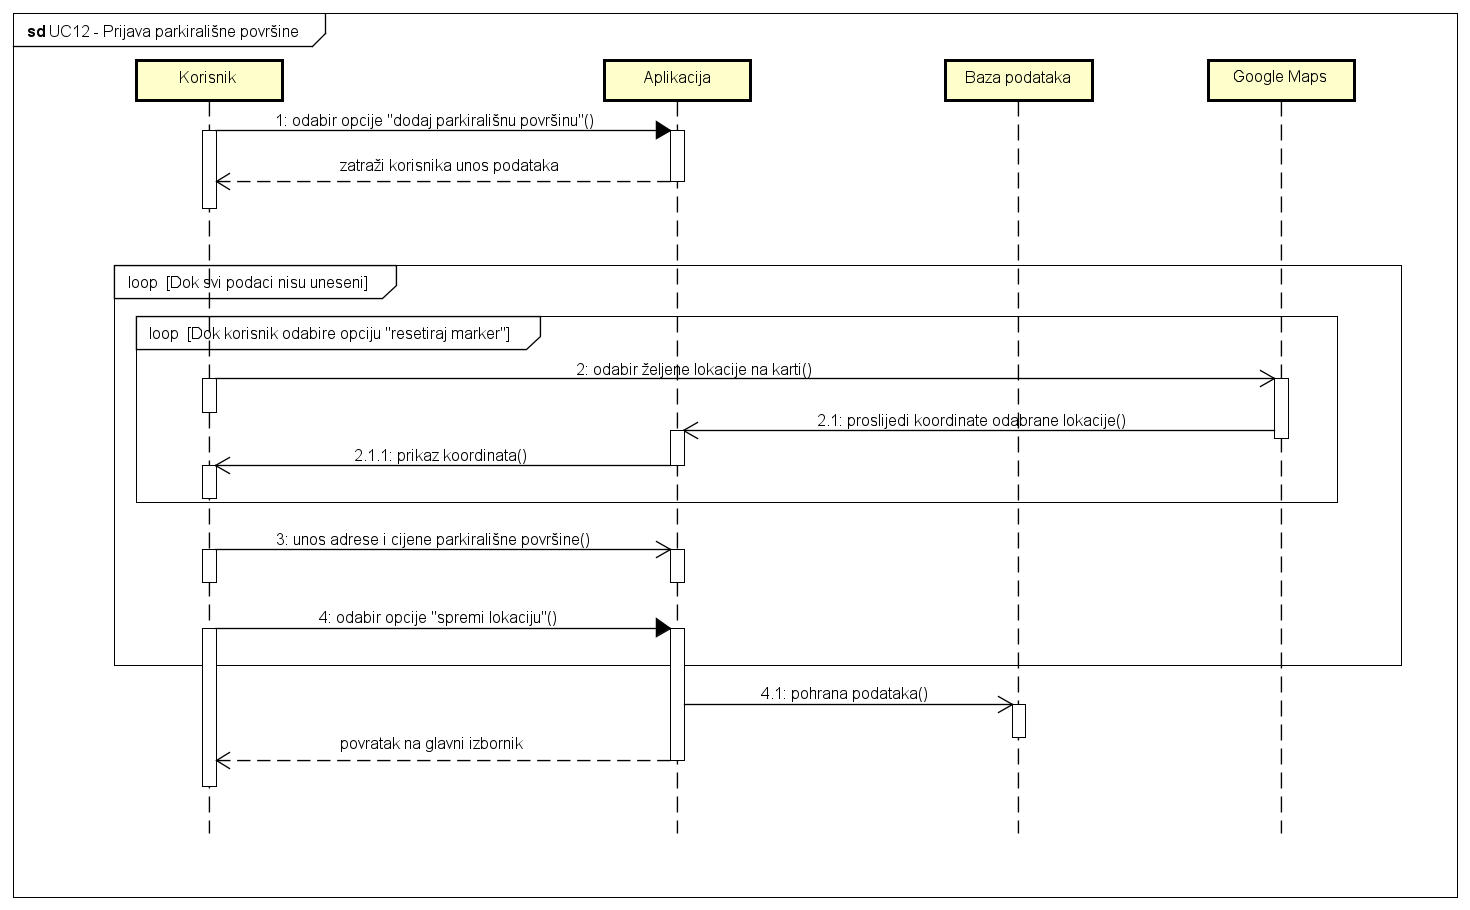
\includegraphics[scale=0.4]{dijagrami/sekvencijski dijagram - prijava parkirališne površine.png} %veličina slike u odnosu na originalnu datoteku i pozicija slike
				\centering
				\caption{Sekvencijski dijagram - prijava parkirališne površine}
				\label{fig:promjene}
			\end{figure}
			
				\newpage
				\noindent {\textbf{Obrazac uporabe UC17 - Brisanje vozača}}\\
				Administrator može pregledati i upravljati svim vozačima. Odabirom opcije "Popis vozača" prikazuje se lista svih prijavljenih vozača. Klikom na gumb "Obriši" pored željenog vozača, aplikacija pristupa bazi podataka i uklanja ga. Baza podataka šalje novi popis prijavljenih vozača, aplikacija se ažurira i prikazuje novu listu svih vozača.
			 \\
		
				\begin{figure}[H]
					\includegraphics[scale=0.5]{dijagrami/Sekvencijski dijagram - brisanje vozača.png} %veličina slike u odnosu na originalnu datoteku i pozicija slike
					\centering
					\caption{Sekvencijski dijagram - brisanje vozača}
					\label{fig:promjene}
				\end{figure}		
				
				\eject
	
		\section{Ostali zahtjevi}
			 
			 \begin{packed_item}
			 	
			 	\item  Sustav treba omogućiti rad više korisnika u stvarnom vremenu 
			 	\item  Sustav mora podržavati hrvatsku abecedu koji se mogu pojavljivati u korisničkim imenima i nazivima objekata na karti grada Zagreba
			 	\item  Komunikacija sa bazom podataka (slanje upita i primanje odgovora od baze) ne smije trajati dulje od nekoliko sekundi
			 	\item  Sustav treba biti implementiran kao web aplikacija
			 	\item  Korištenje sustava na način na koji nije zamišljeno ne smije narušiti funkcionalnost i rad
			 	\item  Sustav treba biti intuitivan za korištenje
			 	\item  Nadogradnja sustava provodi se na temelju zadnje verzije bez mijenjanja ključnih dijelova sustava
			 	\item Sustav kao valutu treba podržati HRK
			 	\item Cijene rezervacija prikazuju točan iznos do drugog decimalnog mjesta
			 	\item Baza podataka treba biti otporna na napade i greške
			 	\item Pristup sustavu treba biti omogućen iz javne mreže pomoću HTTPS-a
			 	\item Sustav korisniku mora omogućiti registraciju neograničenog broja automobila
			 	\item Lokacija parkirališnih površina ima odstupanje od maksimalno 30 metara
			 	\item Sustav je dostupan 24 sata dnevno, 365 dana u godini (osim u trenucima obnavljanja ili nadogradnje sustava)
			 	
			 \end{packed_item}
			 
	
	